\documentclass[landscape, 8pt, a4paper, oneside]{extarticle}
\usepackage[utf8]{inputenc}
\usepackage[T1]{fontenc}
\usepackage{amssymb}
\usepackage{amsmath}
\usepackage{import}
\usepackage{ifthen}
\usepackage{teamnote}
\usepackage{listings}
\usepackage{xcolor}
\raggedbottom
\usepackage{fontspec}
\usepackage{kotex}
\setmonofont{Monoplex KR Regular}

\teamnote{UCPC}{alreadyallsolved}{already, all, solved}

\ShowUsage
\ShowComplexity
\HideAuthor
\usepackage{etoolbox}
\usepackage{tikz}
\newboolean{BangShowGrid}
\setboolean{BangShowGrid}{false}
\newcommand{\ShowGrid}{\setboolean{BangShowGrid}{true}}
\newcommand{\HideGrid}{\setboolean{BangShowGrid}{false}}

\begin{document} \begin{multicols*}{3}
  \maketitlepage
  
  \section{Basic Implementation}
  \Algorithm{Main Template}{}{}{cpp}{source/0. Basic Implementation/main.cpp}{}
  %\Algorithm{Debug Snippet}{}{}{cpp}{source/0. Basic Implementation/Debug.cpp}{}
  \section{Math}
  \Algorithm{Basic Arithmetic}{}{}{cpp}{source/1. Math/Basic arithmetic.cpp}{}
  \Algorithm{Binomial Coefficient}{}{$O(1)$ / $O(\sum p^k)$}{cpp}{source/1. Math/Binomial Coefficient.cpp}{}
  \Algorithm{Chinese Remainder Theorem}{Solve system of linear congruences.}{$O(\log N)$}{cpp}{source/1. Math/Chinese remainder theorem.cpp}{}
  \Algorithm{FFT \& NTT}{Fast Fourier/Number Theoretic Transform for convolutions.}{$O(N \log N)$}{cpp}{source/1. Math/FFT + NTT.cpp}{}
  \Algorithm{Bostan-Mori}{}{$O(d \log d \log k)$}{cpp}{source/1. Math/bostan_mori.cpp}{}
  \Algorithm{Linear Sieve}{Find primes and multiplicative functions in linear time.}{$O(N)$}{cpp}{source/1. Math/Linear Sieve.cpp}{}
  \Algorithm{Miller-Rabin \& Pollard-Rho}{Primality test and integer factorization.}{$O(\log^3 N) / O(N^{1/4})$}{cpp}{source/1. Math/Miller rabin + Pollard rho.cpp}{}
  \Algorithm{XOR Basis}{}{}{cpp}{source/1. Math/XOR Basis.cpp}{}
  \Algorithm{Floor Sum}{$\sum_{k=1}^{n} \lfloor n/k \rfloor$}{}{cpp}{source/1. Math/Floor Sum.cpp}{}
  \Algorithm{Xuduh Sieve}{Calculate prefix sum of multiplicative function}{$O(N^{3/4})$}{cpp}{source/1. Math/Xudyh Sieve.cpp}{}
  \Algorithm{Discrete Log}{}{$O(\sqrt{P} \log P)$}{cpp}{source/1. Math/Discrete Log.cpp}{}
  %\Algorithm{}{}{}{python}{source/1. Math/Discrete Log.py}{}
  \Algorithm{Multiplicative Order}{Find the minimum positive $k$ s.t. $a^k \equiv 1 \pmod mod$)}{}{cpp}{source/1. Math/Multiplicative Order.cpp}{}
  %\Algorithm{}{}{}{python}{source/1. Math/Multiplicative Order.py}{}
  \Algorithm{Power Tower}{}{}{cpp}{source/1. Math/Power Tower.cpp}{}
  %\Algorithm{}{}{}{python}{source/1. Math/Power Tower.py}{}
  \Algorithm{Simplex}{}{}{cpp}{source/1. Math/Simplex.cpp}{}
  
  \section{Data Structure}
  \Algorithm{Erasable Priority Queue}{}{}{cpp}{source/2. Data structure/Erasable PQ.cpp}{}
  \Algorithm{Non-Recursive Segment Tree}{}{}{cpp}{source/2. Data structure/NonRec_SegTree.cpp}{}
  \Algorithm{Inversion counting}{}{}{cpp}{source/2. Data structure/Inversion counting.cpp}{}
  \Algorithm{1D \& 2D Fenwick Tree}{Point updates and subgrid sums on a 2D plane.}{1D: $O(\log N)$, 2D: $O(\log N \log M)$}{cpp}{source/2. Data structure/Fenwick-tree.cpp}{}
  \Algorithm{Merge Sort Tree}{Count/rank of elements in range $[L, R]$.}{$O(\log^2 N)$ per query}{cpp}{source/2. Data structure/MergeSortTree.cpp}{}
  \Algorithm{Persistent Segment Tree}{Accessing previous versions and range k-th element.}{$O(\log N)$ per query}{cpp}{source/2. Data structure/PersistentSegmentTree.cpp}{}
  %\Algorithm{Sweepline Mo's}{Optimized Mo's for $O(1)$ update and $O(1)$ query via offline sweepline.}{$O(N\sqrt{Q})$}{cpp}{source/2. Data structure/Sweepline MOs.cpp}{}
  \Algorithm{Link-Cut Tree}{Dynamic tree structure supporting link, cut, and path operations using auxiliary Splay trees.}{Amortized $O(\log N)$}{cpp}{source/2. Data structure/LinkCutTree.cpp}{}
  \Algorithm{Li Chao Tree}{}{}{cpp}{source/2. Data structure/Li chao tree.cpp}{}
  %\Algorithm{Lazy Segment Tree}{}{}{cpp}{source/2. Data structure/Lazy segtree.cpp}{}
  \Algorithm{DSU (Weighted)}{}{}{cpp}{source/2. Data structure/DSU (Weighted).cpp}{}
  \Algorithm{Trie}{}{}{cpp}{source/2. Data structure/Trie.cpp}{}

  \section{Graph}
  \Algorithm{Bellman Ford}{SSSP with negative weights/cycles.}{$O(VE)$}{cpp}{source/3. Graph/Bellman.cpp}{}
  %\Algorithm{SPFA (SLF Optimized)}{SSSP with negative weights. Returns false if negative cycle detected.}{Avg $O(E)$, Worst $O(VE)$}{cpp}{source/3. Graph/SPFA.cpp}{}
  \Algorithm{LCA}{Lowest Common Ancestor using binary lifting.}{$O(\log N)$}{cpp}{source/3. Graph/LCA.cpp}{}
  \Algorithm{HLD}{Heavy-Light Decomposition for path queries on trees.}{$O(\log^2 N)$}{cpp}{source/3. Graph/HLD.cpp}{}
  \Algorithm{Centroid Decomposition}{Divide and conquer on trees for path/distance problems.}{$O(N \log N)$ build}{cpp}{source/3. Graph/Centroid Decomposition.cpp}{}
  \Algorithm{Bipartite Matching}{Maximum matching in bipartite graphs.}{$O(E\sqrt{V})$}{cpp}{source/3. Graph/Bipartite_Matching.cpp}{}
  \Algorithm{Hungarian}{}{$O(N^3)$}{cpp}{source/3. Graph/Hungarian.cpp}{}
  \Algorithm{Dinic}{Efficient maximum flow algorithm.}{$O(V^2E)$}{cpp}{source/3. Graph/Dinic.cpp}{}
  \Algorithm{MCMF}{Minimum Cost Maximum Flow.(zkw MCMF)}{$O(F \cdot E \log V)$}{cpp}{source/3. Graph/MCMF.cpp}{}
  \Algorithm{Circulation}{Flow with lower and upper bounds.}{}{cpp}{source/3. Graph/Circulation.cpp}{}
  \Algorithm{SCC}{Strongly Connected Components.}{$O(V+E)$}{cpp}{source/3. Graph/SCC.cpp}{}
  \Algorithm{2-sat}{Solves 2-SAT in $O(V+E)$; $x_i$ is true if $SCC(x_i) < SCC(\neg x_i)$.}{$O(V+E)$}{cpp}{source/3. Graph/two-sat.cpp}{}
  \Algorithm{BCC}{Biconnected Components, Cut-vertices, and Bridges.}{$O(V+E)$}{cpp}{source/3. Graph/BCC.cpp}{}
  \Algorithm{Find 3 or 4 cycle}{Finds all $C_3$ and $C_4$ cycles using degree ordering.}{$O(M\sqrt{M})$}{cpp}{source/3. Graph/Find34Cycle.cpp}{}
  \Algorithm{Push Relabel}{Max flow via preflow-push and labeling}{$O(V^3)$}{cpp}{source/3. Graph/PushRelabel.cpp}{}
  \Algorithm{Gomory Hu Tree}{}{}{cpp}{source/3. Graph/Gomory Hu Tree.cpp}{}
  \Algorithm{General Matching}{Maximum Unweighted Matching.}{$O(N^3)$}{cpp}{source/3. Graph/General_Matching.cpp}{}
  %\Algorithm{Weighted General Matching}{Maximum Weighted Matching.}{$O(N^3)$}{cpp}{source/3. Graph/Weighted_General_Matching.cpp}{}
  
  \section{DP Optimization}
  \Algorithm{Convex Hull Trick}{\texttt{dp[i] = min(dp[j] + b[j] * a[i]), b[j] >= b[j+1]}}{$O(N \log N)$}{cpp}{source/4. DP/Convex Hull Trick.cpp}{}
  \Algorithm{Linear CHT}{CHT when slopes(k)/queries(x) are monotonic.}{$O(N)$}{cpp}{source/4. DP/Linear CHT.cpp}{}
  \Algorithm{D\&C optimization}{\texttt{dp[t][i] = min(dp[t-1][j] + c[j][i]), c is Monge}}{$O(KN \log N)$}{cpp}{source/4. DP/DNC opt.cpp}{}
  \Algorithm{Monotone Queue optimization}{\texttt{dp[i] = min(dp[j] + c[j][i]), c is Monge,\ find cross}}{$O(N \log N)$}{cpp}{source/4. DP/MonotoneQueue opt.cpp}{}
  \Algorithm{Aliens Trick}{\texttt{dp[t][i] = min(dp[t-1][j] + c[j+1][i]), c is Monge, find lambda w/ half bs}}{$O(T \log X)$}{cpp}{source/4. DP/Aliens.cpp}{}
  \Algorithm{Sum Over Subsets}{\texttt{dp[mask] = sum(A[i]), i is in mask}}{$O(N2^N)$}{cpp}{source/4. DP/SumOverSubsets.cpp}{}
  \Algorithm{Berlekamp Massey}{Linear recurrence $N$-th term. Sparse matrix determinant.}{$N$-th term: $O(K^2 \log N)$ / Det: $O(N(N+E))$}{cpp}{source/4. DP/Berlekamp_massey.cpp}{}
  
  \section{Geometry}
  \Algorithm{Geometry Template}{Basic point, line, and circle operations.}{}{cpp}{source/5. Geometry/Basic Template.cpp}{}
  \Algorithm{Closest Pair}{}{$O(N \log N)$}{cpp}{source/5. Geometry/Closest Pair.cpp}{}
  \Algorithm{Convex Hull}{Finds the convex hull using Monotone Chain. Returns vertices in CCW order.}{$O(N \log N)$}{cpp}{source/5. Geometry/ConvexHull.cpp}{}
  \Algorithm{Convex Hull 3d}{}{$O(N^2)$}{cpp}{source/5. Geometry/ConvexHull 3D.cpp}{}
  \Algorithm{Rotating Calipers}{Calculates the diameter (farthest pair of points) of a convex hull(CCW order).}{$O(N)$}{cpp}{source/5. Geometry/Calipers.cpp}{}
  \Algorithm{Point in Convex Polygon}{Checks if a point is inside or on the boundary of a convex polygon (CCW sorted).}{$O(\log N)$}{cpp}{source/5. Geometry/PointInConvexPolygon.cpp}{}
  \Algorithm{Point in Polygon}{Ray casting algorithm for general polygons.}{$O(N)$}{cpp}{source/5. Geometry/PointInPolygon.cpp}{}
  \Algorithm{Sort Points}{Angular sort. 1. Relative to pivot (Convex Hull). 2. Relative to origin.}{}{cpp}{source/5. Geometry/SortPoints.cpp}{}
  \Algorithm{Linear Minkowski Sum}{Minkowski Sum of Two convex(must be CCW order).}{$O(N+M)$}{cpp}{source/5. Geometry/LinearMinkowski.cpp}{}
  \Algorithm{Polygon Area}{Calculates 2 $\times$ Area of a polygon (Shoelace formula).}{$O(N)$}{cpp}{source/5. Geometry/PolygonArea.cpp}{}
  \Algorithm{Smallest Enclosing Circle}{Welzl's algorithm to find the Minimum Enclosing Circle. Returns {center, radius}.}{Expected $O(N)$}{cpp}{source/5. Geometry/EnclosingCircle.cpp}{}
  \Algorithm{Geometric Intersections}{Intersection primitives: Segment, Line-Circle, Line-Hull, and Circle-Polygon area.}{$O(1) / O(1) / O(\log N) / O(N)$}{cpp}{source/5. Geometry/Intersect.cpp}{}
  \Algorithm{Half Plane Intersection}{Intersection of half-planes defined by lines (left side is valid). Returns a convex polygon.}{$O(N \log N)$}{cpp}{source/5. Geometry/HalfPlaneIntersect.cpp}{}
  \Algorithm{Manhattan MST}{}{$O(N \log N)$}{cpp}{source/5. Geometry/manhattan_mst.cpp}{}
  \Algorithm{Shamos-Hoey}{}{$O(N \log N)$}{cpp}{source/5. Geometry/shamos_hoey.cpp}{}
  
  \section{String}
  \Algorithm{Aho-Corasick}{Multi-pattern matching using trie and failure links.}{$O(\sum |P| + |T|)$}{cpp}{source/6. String/Aho-Corasick.cpp}{}
  \Algorithm{Hashing}{Rolling hash for string matching.}{$O(N)$}{cpp}{source/6. String/Hashing.cpp}{}
  \Algorithm{KMP}{Single pattern matching using prefix function.}{$O(N+M)$}{cpp}{source/6. String/KMP.cpp}{}
  \Algorithm{Manacher}{Find all palindromic substrings in linear time.}{$O(N)$}{cpp}{source/6. String/Manacher.cpp}{}
  \Algorithm{Suffix Array}{Suffix array and LCP array.}{$sa: O(N \log N), lcp: O(N)$}{cpp}{source/6. String/SuffixArray.cpp}{}
  \Algorithm{Z-algorithm}{Longest common prefix between S and its suffixes.}{$O(N)$}{cpp}{source/6. String/Z.cpp}{}
  \Algorithm{Eertree}{Manages all distinct palindromic substrings using length and suffix links.}{$O(N \log \Sigma)$}{cpp}{source/6. String/eertree.cpp}{}
  \Algorithm{Suffix Automaton}{Builds a DFA representing all substrings. Supports substring counting and pattern matching.}{$O(N \cdot \Sigma)$}{cpp}{source/6. String/SuffixAutomaton.cpp}{}
  
  \section{STL \& pbds}
  \Algorithm{Hash map (pb\_ds)}{Faster hash table using pb\_ds.}{$O(1)$}{cpp}{source/7. STL + pbds/Hash map(pbds).cpp}{}
  \Algorithm{Ordered Set (pb\_ds)}{Set supporting order\_of\_key and find\_by\_order.}{$O(\log N)$}{cpp}{source/7. STL + pbds/Ordered Set(pbds).cpp}{}
  \Algorithm{Permutation \& Combination}{next\_permutation and mask-based combinations.}{}{cpp}{source/7. STL + pbds/Permutation + Combination.cpp}{}
  \Algorithm{Priority Queue (pb\_ds)}{Meldable heap supporting modify/erase via point\_iterator.}{$O(\log N)$}{cpp}{source/7. STL + pbds/Priority queue(pbds).cpp}{}
  \Algorithm{Rope}{Persistent sequence supporting fast insertion, deletion and slicing.}{$O(\log N)$}{cpp}{source/7. STL + pbds/Rope.cpp}{}
  %\Algorithm{Trie (pb\_ds)}{Prefix tree implementation from pb\_ds.}{}{cpp}{source/7. STL + pbds/Trie(pbds).cpp}{}
  
  \section{Misc}
  \Algorithm{Custom Hash}{Custom hash for pair, vector.}{}{cpp}{source/8. Misc/Custom hash.cpp}{}
  \Algorithm{Fast I/O}{Fast integer I/O using fread/fwrite.}{}{cpp}{source/8. Misc/Fastio.cpp}{}
  \Algorithm{Random}{Better random for mt19937.}{}{cpp}{source/8. Misc/Random.cpp}{}
  \Algorithm{Ternary Search}{Finding extremum of unimodal functions.}{$O(\log N)$}{cpp}{source/8. Misc/Ternary search.cpp}{}
  \Algorithm{Some tricks}{Collection of bitwise hacks and optimization techniques.}{}{cpp}{source/8. Misc/Some tricks.cpp}{}
  
  \section{Checklist + Useful Info}
  
  % source: https://github.com/koosaga/DeobureoMinkyuParty/blob/master/teamnote.tex
  \Algorithm{Highly Composite Numbers, Large Prime}{}{}{}{}{}
  \input{source/8. Misc/Primes}
  
  \linespread{1.1}
  % source: https://github.com/green5555/Teamnote-archive/blob/main/2020%20ICPC%20-%20Gr-Yee-n55/code/useful.txt
  %         https://github.com/overnap/cp-teamnote/blob/master/tn.tex
  % edit by alreadysolved
  \Algorithm{Useful Stuff}{}{}{}{}{}
  \begin{itemize}
    \item Catalan Number\\
    1, 1, 2, 5, 14, 42, 132, 429, 1430, 4862, 16796, 58786, 208012, 742900\\
    $C_n = \binom{2n}{n} / (n + 1);$\\
    $C_n = \sum_{i=0}^{n-1} C_i \times C_{n-1-i};$\\
    - 길이가 2n인 올바른 괄호 수식의 수\\
    - n + 1개의 리프를 가진 풀 바이너리 트리의 수\\
    - n + 2각형을 n개의 삼각형으로 나누는 방법의 수\\
    - n*n 격자에서 0,0부터 n,n까지 이동할 때, y=x(대각선)를 넘지않고 우상단으로만 이동하는 경로의 수\\
    - n개의 노드로 이루어진 이진 트리 구조 개수\\
    - 1부터 n까지의 수를 스택에 넣고 빼서 만들 수 있는 순열의 개수\\
    - 원 위에 2n개의 점이 있고, 2개씩 짝지어 선분을 그었을때 어떤 선분도 교차하지 않는 방법의 수\\
    - $(0,0)$에서 $(N,M)$까지 우상단으로 이동할 때, 직선 $y = x + k$($k>0$)에 닿지않는 경로의 수:
      전체 경로 수 - 반사된 경로 수 = $\binom{N+M}{N} - \binom{N+M}{N-k}$ (직선 $y = x + k$에 처음 닿은 이후 경로를 $y = x + k$에 대해 대칭 이동 -> $(M-k, N+k)$로 매핑됨)
    \item Derangements\\
    N명의 사람이 모자를 벗어두었다가 무작위로 하나씩 집었을 때, 아무도 자기 모자를 쓰지 않을 경우의 수\\
    - 포함배제 ($D_N = N! \sum_{i=0}^N \frac{(-1)^i}{i!}$) - 팩토리얼 역원 전처리로 O(N)\\
    - DP ($D_N = (N-1) \times (D_{N-1} + D_{N-2})$ (단, $D_0=1, D_1=0$)) - O(N) dp 테이블을 만들어두면 쿼리 당 O(1)\\
    - 부분 교란 순열: $N$명 중 정확히 $K$명만 자기 모자를 쓰고, 나머지 $N-K$명은 아무도 자기 모자를 쓰지 않을 경우의 수 - $\binom{N}{K} \times D_{N-K}$
    \item Stars and Bars\\
    N개의 구별되지 않는 물건을 K개의 구별되는 상자에 나누어담는 경우의 수 (빈 상자 허용) - $\binom{N+K-1}{K-1}$\\
    - $x_1 + x_2 + \dots + x_K = N$ ($x_i \ge 0$)의 해의 개수를 구하는 것과 동일\\
    - 각 상자에 적어도 1개 이상 담아야 한다($x_i \ge 1$): 미리 1개씩 나눠줌. $N'=N-K$로 치환해 $\binom{N'+K-1}{K-1} = \binom{N-1}{K-1}$ 계산\\
    - 어떤 상자도 $C$개를 초과할 수 없다($x_i \le C$): 포함배제와 결합. (조건을 위반하는 상자를 1개, 2개 선택하는 경우를 빼고 더함)
    \item 제2종 스털링 수\\
    서로 다른 $N$개의 물건을 구별되지 않는 $K$개의 상자에 빈 상자 없이 나누어 담는 경우의 수 ($S(N, K)$ 혹은 $\left\{ \begin{matrix} N \\ K \end{matrix} \right\}$)\\
    - 점화식: $S(N, K) = K \times S(N-1, K) + S(N-1, K-1)$ (단, $S(N, 1) = S(N, N) = 1$)\\
    - 직접 계산: $S(N, K) = \frac{1}{K!} \sum_{i=0}^K (-1)^{K-i} \binom{K}{i} i^N$ (단일 행 계산 시 $O(K \log N)$)\\
    - Bell Number ($B_N = \sum_{k=1}^N S(N, k)$): 서로 다른 $N$개의 원소를 분할하는 모든 방법의 수.\\
    - Bell Number 초항: 1, 1, 2, 5, 15, 52, 203, 877, 4140, 21147, 115975
    \item 자연수의 분할\\
    서로 같은 $N$개의 물건을 구별되지 않는 $K$개의 상자에 빈 상자 없이 나누어 담는 경우의 수 ($P(N, K)$)\\
    - 자연수 $N$을 $K$개의 자연수의 합으로 나타내는 방법의 수와 동일.\\
    - 점화식: $P(N, K) = P(N-1, K-1) + P(N-K, K)$\\
    - $P(N) = \sum_{k=1}^N P(N, k)$: 자연수 $N$의 총 분할 수. \\
    - $P(N)$ 초항: 1, 1, 2, 3, 5, 7, 11, 15, 22, 30, 42, 56, 77, 101, 135
    \item Cayley's Formula \& Prüfer Sequence\\
    $N$개의 구별되는 정점으로 만들 수 있는 서로 다른 스패닝 트리의 개수 = $N^{N-2}$\\
    - 각 정점의 차수가 $d_1, d_2, \dots, d_N$으로 고정되었을 때 가능한 트리의 개수 = $\frac{(N-2)!}{(d_1-1)!(d_2-1)! \dots (d_N-1)!}$ (단, $\sum d_i = 2N-2$)
    \item Binomial Identities\\
    시그마가 포함된 조합론 수식을 $O(1)$로 단순화할 때 사용.\\
    - Hockey-stick Identity (파스칼의 삼각형 대각선 합): $\sum_{i=K}^N \binom{i}{K} = \binom{N+1}{K+1}$\\
    - Vandermonde's Identity (두 집합에서 뽑기): $\sum_{i=0}^K \binom{N}{i}\binom{M}{K-i} = \binom{N+M}{K}$\\
    - 제곱의 합: $\sum_{i=0}^N \binom{N}{i}^2 = \binom{2N}{N}$
    \item Fibonacci Identities\\
    - Cassini's identity: $F_{n-1}F_{n+1} - F_n^2 = (-1)^n$\\
    - Addition formula: $F_{n+k} = F_k F_{n+1} + F_{k-1} F_n$\\
    - Zeckendorf's theorem: 모든 양의 정수는 연속하지 않는 피보나치 수들의 합으로 유일하게 표현 가능하며, 이는 그리디하게 큰 피보나치 수부터 빼는 것으로 구할 수 있다.
    \item Möbius Inversion\\
    - $g(n) = \sum_{d|n} f(d) \iff f(n) = \sum_{d|n} \mu(d)g(n/d)$\\
    - $g(n) = \sum_{n|d} f(d) \iff f(n) = \sum_{n|d} \mu(d/n)g(d)$
    \item Burnside’s Lemma\\
    경우의 수를 세는데, 특정 transform operation(회전, 반사, ..) 해서 같은 경우들은 하나로 친다. 전체 경우의 수는? 각 operation마다 이 operation을 했을 때 변하지 않는 경우의 수를 센다 (단, “아무것도 하지 않는다” 라는 operation도 있어야 함!) 전체 경우의 수를 더한 후, operation의 수로 나눈다. (답이 맞다면 항상 나누어 떨어져야 한다)
    \item 알고리즘 게임\\
    - Nim Game의 해법: 각 더미의 돌의 개수를 모두 XOR했을 때 0이 아니면 첫번째, 0이면 두번째 플레이어가 승리.\\
    - Grundy Number: 어떤 상황의 Grundy Number는, 가능한 다음 상황들의 Grundy Number를 모두 모은 다음, 그 집합에 포함 되지 않는 가장 작은 수가 현재 state의 Grundy Number가 된다. 만약 다음 state가 독립된 여러개의 state들로 나뉠 경우, 각각의 state의 Grundy Number의 XOR 합을 생각한다.\\
    - Subtraction Game: 한 번에 k 개까지의 돌만 가져갈 수 있는 경우, 각 더미의 돌의 개수를 k + 1로 나눈 나머지를 XOR 합하여 판단한다.\\
    - Index-k Nim: 한 번에 최대 k개의 더미를 골라 각각의 더미에서 아무렇게나 돌을 제거할 수 있을 때, 각 binary digit에 대하여 합을 k + 1로 나눈 나머지를 계산한다. 만약 이 나머지가 모든 digit에 대하여 0이라면 두번째, 하나라도 0이 아니라면 첫번째 플레이어가 승리.
    - Misere Nim: 모든 돌 무더기가 1이면 N이 홀수일 때 후공 승, 그렇지 않은 경우 XOR 합 0이면 후공 승
    \item Pick’s Theorem\\
    격자점으로 구성된 simple polygon이 주어짐. I 는 polygon 내부의 격자점 수, B 는 polygon 선분 위 격자점 수, A는 polygon의 넓이라고 할 때, 다음과 같은 식이 성립한다. $A=I+B/2-1$
    \item 가장 가까운 두 점: 분할정복으로 가까운 6개의 점만 확인
    \item 홀의 결혼 정리: 이분그래프(L-R)에서, 모든 L을 매칭하는 필요충분 조건 = L에서 임의의 부분집합 S를 골랐을 때, 반드시 (S의 크기) $\le$ (S와 연결되어있는 모든 R의 크기)이다.
    \item 소수: 10 007 , 10 009 , 10 111 , 31 567 , 70 001 , 1 000 003 , 1 000 033 , 4 000 037 , 99 999 989 , 999 999 937 , 1 000 000 007 , 1 000 000 009 , 9 999 999 967 , 99 999 999 977
    \item 소수 개수 : (1e5 이하 : 9592), (1e7 이하 : 664 579) , (1e9 이하 : 50 847 534)
    \item $10^{15}$ 이하의 정수 범위의 나눗셈 한번은 오차가 없다.
    \item N의 약수의 개수 = $O(N^{1/3})$, N의 약수의 합 = $O(N \log \log N)$
    \item $\phi(mn) = \phi(m) \phi(n) , \phi(pr^n) = pr^n - pr^{n-1} , a^{\phi(n)} \equiv 1 \pmod{n} \ \text{if coprime}$
    \item Euler characteristic : v - e + f (면, 외부 포함) = 1 + c (컴포넌트)
    \item Euler's phi $\phi (n)=n\prod _{p\mid n}\left(1-{\frac {1}{p}}\right)$
    \item Lucas' Theorem $\binom{m}{n}=\prod\binom{m_i}{n_i} \pmod p$ $m_i$, $n_i$는 $p^i$의 계수
    \item 스케줄링에서 데드라인이 빠른 걸 쓰는게 이득. 늦은 스케줄이 안들어갈 때 가장 시간 소모가 큰 스케줄 1개를 제거하면 이득.
  \end{itemize}
  
  % source: https://github.com/justiceHui/icpc-teamnote/blob/master/code/Notes/Checklist.tex
  %         https://github.com/overnap/cp-teamnote/blob/master/tn.tex
  \Algorithm{자주 쓰이는 문제 접근법}{}{}{}{}{}
  \begin{itemize}
    \item 비슷한 문제를 풀어본 적이 있던가?
    \item 단순한 방법에서 시작할 수 있을까? (brute force)
    \item 내가 문제를 푸는 과정을 수식화할 수 있을까? (예제를 직접 해결해보면서)
    \item 문제를 단순화할 수 없을까? / 그림으로 그려볼 수 있을까?
    \item 수식으로 표현할 수 있을까? / 문제를 분해할 수 있을까?
    \item 뒤에서부터 생각해서 문제를 풀 수 있을까? / 순서를 강제할 수 있을까?
    \item 특정 형태의 답만을 고려할 수 있을까? (정규화)
    \item 구간을 통째로 가져간다 : 플로우 + 적당한 자료구조\\$(i,i+1,k,0),(s,e,1,w),(N,T,k,0)$
    \item 말도 안 되는 것 / 당연하다고 생각한 것 다시 생각해 보기
    \item 특수 조건을 꼭 활용 / 여사건으로 생각하기
    \item 게임이론 - 거울 전략 혹은 mex DP 연계
    \item 겁먹지 말고 경우 나누어 생각 / 해법에서 역순으로 가능한가?
    \item 딱 맞는 시간복잡도에 집착하지 말자 / 문제에 의미있는 작은 상수 이용
    \item 스몰투라지, 트라이, 해싱, 루트질 같은 트릭 생각
    \item 너무 추상화하기보단 풀려야 하는 방식으로 생각하기
    \item 잘못된 방법으로 파고들지 말고 버리자 / 제발 터널 비전에 빠지지 말자
    \item 헬프 콜은 적극적으로 / 혼자 멘탈 나가지 않기
  \end{itemize}
  
  % source: https://github.com/overnap/cp-teamnote/blob/master/tn.tex
  \Algorithm{DP 최적화 접근}{}{}{}{}{}
  \begin{itemize}
    \item C[i, j] = A[i] * B[j]이고 A, B가 단조증가, 단조감소이면 Monge
    \item l..r의 값들의 sum이나 min은 Monge
    \item 식 정리해서 일차(CHT) 혹은 비슷한(MQ) 함수를 발견, 구현 힘들면 Li-Chao
    \item $a \le b \le c \le d$에서 $A[a,c] + A[b,d] \le A[a,d] + A[b,c]$
    \item Monge 성질을 보이기 어려우면 $N^2$ 나이브 짜서 opt의 단조성을 확인하고 찍맞
    \item 식이 간단하거나 변수가 독립적이면 DP 테이블을 세그 위에 올려서 해결
    \item 침착하게 점화식부터 세우고 Monge인지 판별
    \item Monge에 집착하지 말고 단조성이나 볼록성만 보여도 됨
  \end{itemize}
  
  % source: https://github.com/justiceHui/icpc-teamnote/blob/master/code/Notes/MinCut.tex
  \Algorithm{Graph Matching(Graph with $\vert V \vert \leq 500$)}{}{}{}{}{}
  \begin{itemize}
    \item \textbf{Game on a Graph} : $s$에 토큰이 있음. 플레이어는 각자의 턴마다 토큰을 인접한 정점으로 옮기고 못 옮기면 짐.\\
    $s$를 포함하지 않는 최대 매칭이 존재함 $\leftrightarrow$ 후공이 이김
    \item \textbf{Chinese Postman Problem} : 모든 간선을 방문하는 최소 가중치 Walk를 구하는 문제.\\
    Floyd를 돌린 다음, 홀수 정점들을 모아서 최소 가중치 매칭 (홀수 정점은 짝수 개 존재)
    \item \textbf{Unweighted Edge Cover} : 모든 정점을 덮는 가장 작은(minimum cardinality/weight) 간선 집합을 구하는 문제\\
    $\vert V\vert - \vert M\vert$, 길이 3짜리 경로 없음, star graph 여러 개로 구성
    \item \textbf{Weighted Edge Cover} : $sum_{v \in V}(w(v)) - sum_{(u,v) \in M}(w(u) + w(v) - d(u,v))$, $w(x)$는 $x$와 인접한 간선의 최소 가중치
    \item \textbf{NEERC'18 B} : 각 기계마다 2명의 노동자가 다뤄야 하는 문제.\\
    기계마다 두 개의 정점을 만들고 간선으로 연결하면 정답은 $\vert M\vert - \vert\text{기계}\vert$임. 정답에 1/2씩 기여한다는 점을 생각해보면 좋음.
    \item \textbf{Min Disjoint Cycle Cover} : 정점이 중복되지 않으면서 모든 정점을 덮는 길이 3 이상의 사이클 집합을 찾는 문제.\\
    모든 정점은 2개의 서로 다른 간선, 일부 간선은 양쪽 끝점과 매칭되어야 하므로 플로우를 생각할 수 있지만 용량 2짜리 간선에 유량을 1만큼 흘릴 수 있으므로 플로우는 불가능.\\
    각 정점과 간선을 2개씩($(v, v')$, $(e_{i,u},e_{i,v})$)로 복사하자. 모든 간선 $e=(u,v)$에 대해 $e_u$와 $e_v$를 잇는 가중치 w짜리 간선을 만들고(like NEERC18), $(u,e_{i,u}), (u',e_{i,u}), (v,e_{i,v}), (v',e_{i,v})$를 연결하는 가중치 0짜리 간선을 만들자. Perfect 매칭이 존재함 $\Leftrightarrow$ Disjoint Cycle Cover 존재. 최대 가중치 매칭 찾은 뒤 모든 간선 가중치 합에서 매칭 빼면 됨.
    \item \textbf{Two Matching} : 각 정점이 최대 2개의 간선과 인접할 수 있는 최대 가중치 매칭 문제.\\
    각 컴포넌트는 정점 하나/경로/사이클이 되어야 함. 모든 서로 다른 정점 쌍에 대해 가중치 0짜리 간선 만들고, 가중치 0짜리 $(v,v')$ 간선 만들면 Disjoing Cycle Cover 문제가 됨. 정점 하나만 있는 컴포넌트는 self-loop, 경로 형태의 컴포넌트는 양쪽 끝점을 연결한다고 생각하면 편함.
  \end{itemize}
  
  % source: https://github.com/justiceHui/icpc-teamnote/blob/master/code/Notes/MinCut.tex
  \Algorithm{Mincut 모델링}{}{}{}{}{}
  \begin{itemize}
    \item $N$개의 boolean 변수 $v_1, \cdots, v_n$을 정해서 비용을 최소화하는 문제=true인 점은 $T$, false인 점은 $F$와 연결되게 분할하는 민컷 문제
    \begin{enumerate}
      \item $v_i$가 T일 때 비용 발생: $i$에서 F로 가는 비용 간선
      \item $v_i$가 F일 때 비용 발생: $i$에서 T로 가는 비용 간선
      \item $v_i$가 T이고 $v_j$가 F일 때 비용 발생: $i$에서 $j$로 가는 비용 간선
      \item $v_i \ne v_j$일 때 비용 발생: $i$에서 $j$로, $j$에서 $i$로 가는 비용 간선
      \item $v_i$가 T면 $v_j$도 T여야 함: $i$에서 $j$로 가는 무한 간선
      \item $v_i$가 F면 $v_j$도 F여야 함: $j$에서 $i$로 가는 무한 간선
    \end{enumerate}
    \item 5/6번 + $v_i$와 $v_j$가 달라야 한다는 조건이 있으면 MAX-2SAT
    \item Maximum Density Subgraph (NEERC'06H, BOJ 3611 팀의 난이도)
    \begin{enumerate}
      \item density $\geq x$인 subgraph가 있는지 이분 탐색
      \item 정점 $N$개, 간선 $M$개, 차수 $D_i$개
      \item 그래프의 간선마다 용량 1인 양방향 간선 추가
      \item 소스에서 정점으로 용량 $M$, 정점에서 싱크로 용량 $M-D_i+2x$
      \item min cut에서 S와 붙어 있는 애들이 1개 이상이면 x 이상이고, 그게 subgraph의 정점들
      \item while(r-l $\geq$ 1.0/(n*n)) 으로 해야 함. 너무 많이 돌리면 실수 오차
    \end{enumerate}
  \end{itemize}
  
\end{multicols*}

\ifthenelse{\boolean{BangShowGrid}}{
  \newpage
  \thispagestyle{fancy}
  \noindent 
  \vspace*{-0.5cm} 
  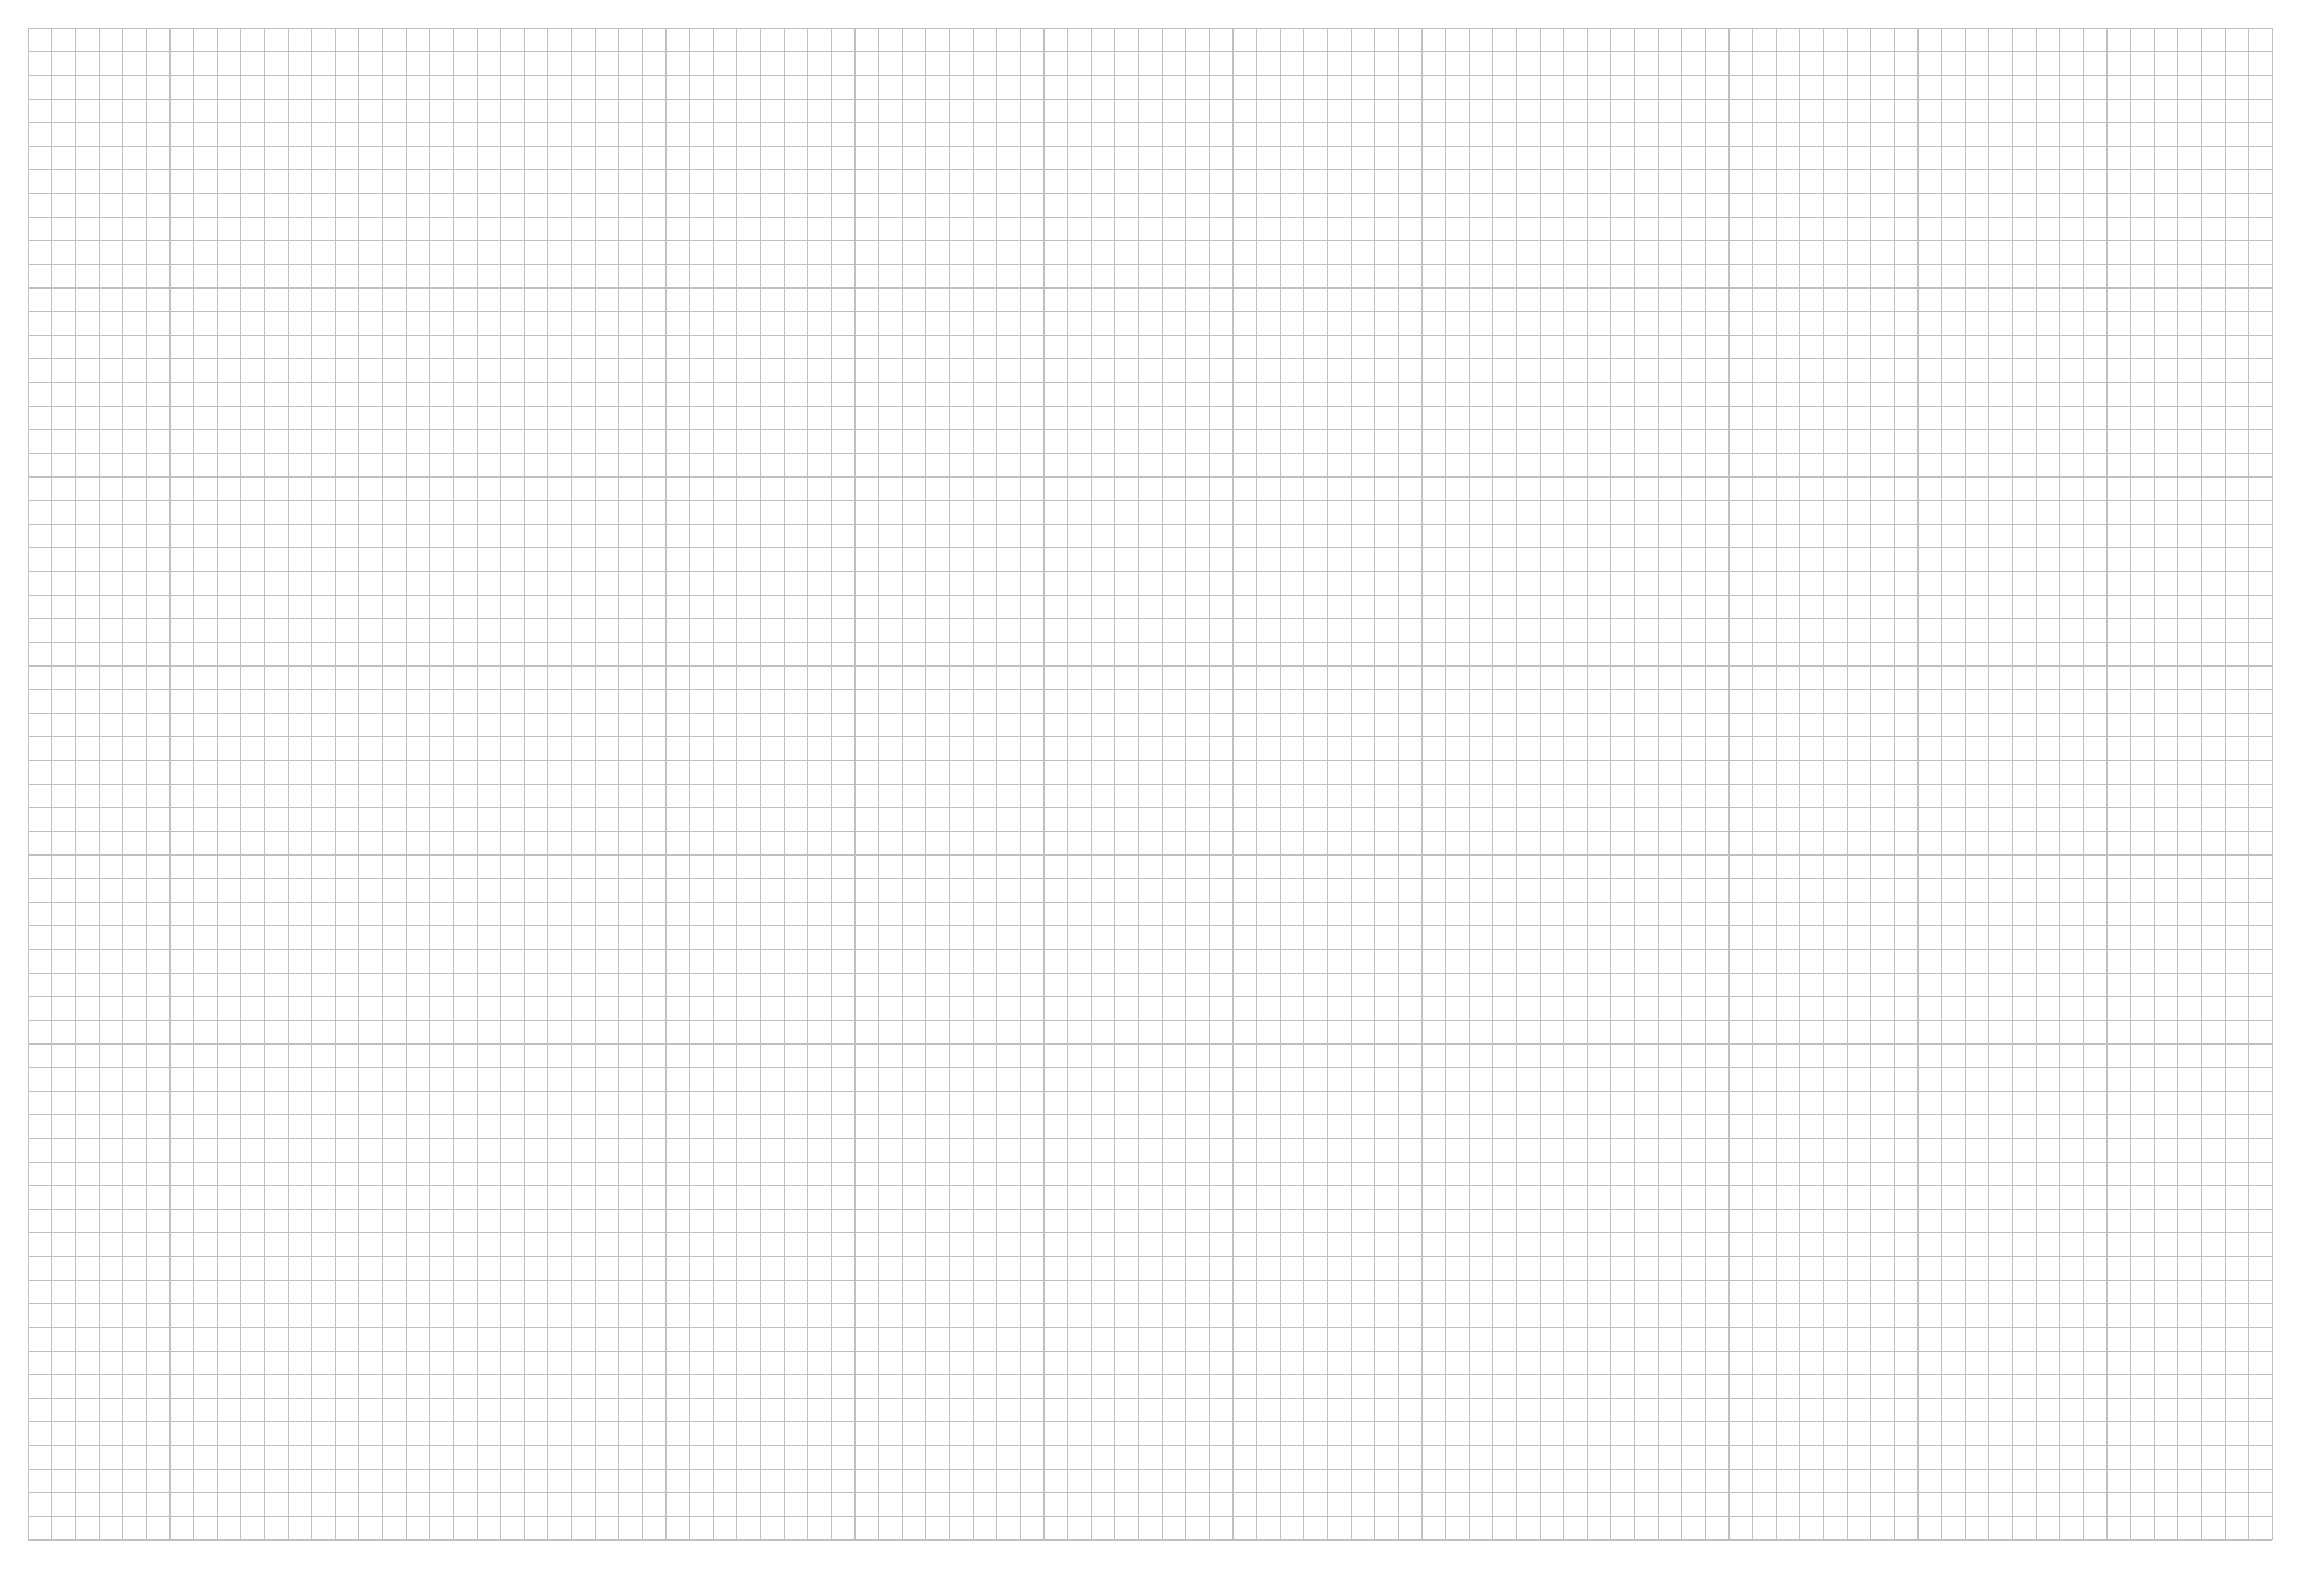
\begin{tikzpicture}
    \draw[step=0.3cm, gray!50, thin] (0,0) grid (28.5, 19.2);
  \end{tikzpicture}
}{}

\end{document}